\clearpage
\phantomsection

\setcounter{chapter}{0}
\chapter[TỔNG QUAN VỀ CÁC PHƯƠNG PHÁP NHẬN DẠNG HỆ THỐNG TRONG TRUYỀN THÔNG KHÔNG DÂY]{Tổng quan về các phương pháp nhận dạng hệ thống trong truyền thông không dây}

Việc nhận dạng hệ thống trong truyền thông không dây đã luôn được phát triển ngay từ những thế hệ mạng không dây đầu tiên~\cite{Tse2005}. Ngày nay, các thuật toán ước lượng kênh truyền không dây đã đạt được các bước tiến đánh kể về độ chính xác và có thể chia thành bốn hướng tiếp cận chính như trên hình~\ref{fig:classify}. Bao gồm sử dụng pilot (Non-blind), mù (B), bán mù (SB), và dựa trên học máy, học sâu (AI-based)~\cite{vilas2022}.

\begin{figure}[H]
    \centering
    \begin{tikzpicture}
        \node (b1) [startstop] at (0, 0) {Các thuật toán ước lượng kênh truyền};

        \node (b21) [process, align=center] at (-60mm, -25mm) {Sử dụng Pilot};

        \node (b22) [process, align=center] at (-20mm, -25mm) {Thuật toán mù};

        \node (b23) [process, align=center] at (20mm, -25mm) {Thuật toán bán mù};

        \node (b24) [process, align=center] at (60mm, -25mm) {Học máy/Học sâu};

        \node (b31) [below=10mm of b21, process, align=left, fill=green!10!white] {
        Least Square (LS) \\
        MMSE~\cite{Jiang2011} \\
        MLE
        };

        \draw[line] (b1.south) -- ([yshift=-5mm]b1.south);
        \draw[arrow] ([yshift=-5mm]b1.south) -| (b21);
        \draw[arrow] ([yshift=-5mm]b1.south) -| (b22);
        \draw[arrow] ([yshift=-5mm]b1.south) -| (b23.north);
        \draw[arrow] ([yshift=-5mm]b1.south) -| (b24.north);

        \draw[arrow] (b21) -- (b31);
        
    \end{tikzpicture}
    \caption{Phân loại các thuật toán ước lượng kênh truyền.}
    \label{fig:classify}
\end{figure}

\section{Mô hình hệ thống MIMO/mMIMO}\label{sec:sm}

This section introduces the mathematical model of MIMO wireless communications used in this work. After that, the MRE algorithm for the MIMO model is briefly reviewed.

\begin{figure}[H]
    \centering
    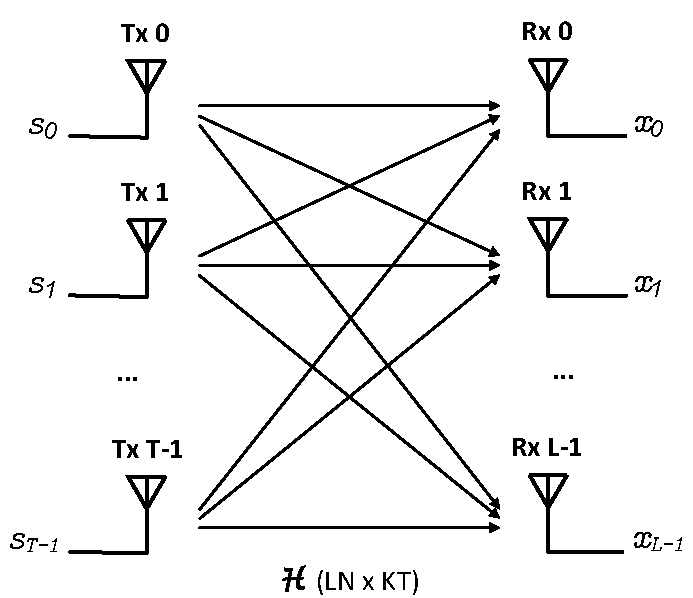
\includegraphics[width=0.6\linewidth]{figures/sys_model.pdf}
    \caption{Mô hình minh hoạ hệ thống truyền trông MIMO.}
    \label{fig:sys_model}
\end{figure}

The MIMO model, illustrated in Fig.~\ref{fig:sys_model}, is composed of
$T$~transmitters and $L$~receivers. Each channel between $t$-th transmitter and $l$-th receiver is formulated as a $M+1$ coefficients vector. At a time, $N$ received symbols are simultaneously captured on each receiver. The following equation expresses the system model
\begin{equation}
    X(i) = \sum_{t=0}^{T-1}\mathcal{H}_t S_t(i) + W_t
\end{equation}
where $S_t(i) \in \mathbb{C}^{M+N \times 1}$ is the transmit symbols from the $t$-th transmitter. $\mathcal{H}_t$ is the channel convolution matrix between $t$-th transmitter and $L$ receivers. $\mathcal{H}_t \in \mathbb{C}^{LN \times K}$ is assumed to be a full column rank ($K = M+N$) matrix. $X(i) \in \mathbb{C}^{LN \times 1}$ denotes the observed signals and $W_t \in \mathbb{C}^{LN \times 1}$ stands for additive white Gaussian noise matrix. Assume that channel and additive noise between each channel are i.i.d and have distributed $\mathcal{CN}(0, \sigma_{\mathcal{H}_t}^2 I)$ and $\mathcal{CN}(0, \sigma^2 I)$, respectively.

\begin{equation*}
    S_t(i) = [s(i), s(i-1),\ldots,s(i-K+1)]^\top
\end{equation*}

\begin{equation*}
    \small
    \mathcal{H}_t= \hspace{-0.7cm}
    \begin{array}{cc}
         & \underset{\longleftrightarrow}{K}\\
         & \left(\begin{array}{cccccc}
    h_0^{(0)} & \cdots & h_M^{(0)} & 0 & \cdots & 0 \\
    \vdots & \cdots & \ddots & \cdots & \ddots & 0 \\
    0 & \cdots & 0 & h_0^{(0)} & \cdots & h_M^{(0)} \\
    \vdots & \cdots & \vdots & \cdots & \cdots & \vdots \\
    h_0^{(L-1)} & \cdots & h_M^{(L-1)} & 0 & \cdots & 0 \\
    \vdots & \cdots & \ddots & \cdots & \ddots & 0 \\
    0 & \cdots & 0 & h_0^{(L-1)} & \cdots & h_M^{(L-1)}
    \end{array}
    \right) 
    \end{array}
    \Big\updownarrow LN    
\end{equation*}

\begin{equation*}
    \begin{aligned}
        X(i) = \big[x^{(0)}(i), \cdots, &x^{(0)}(i-N+1), \cdots, 
        \\ &x^{(L-1)}(i), \cdots, x^{(L-1)}(i-N+1)\big]^\top
    \end{aligned}
\end{equation*} 

\section{Các thuật toán nhận dạng kênh tuyến tính}

\section{Các thuật toán nhận dạng kênh mù}

\section{Các thuật toán nhận dạng kênh bán mù}

\section{Các thuật toán nhận dạng kênh sử dụng học máy}